\chapter{DATA ANALYSIS AND BACKGROUND ESTIMATION METHODS}
\label{chap:DataAnalysis}

\section{Overview}

There are several standard model processes that can mimic our signal events. The largest background contribution comes from quantum chromodynamics (QCD) processes. These are primarily multi-jet events, where electromagnetically-rich jets are misidentified as photons, but can also include processes with true photons either from associated photon production or initial-state radiation. In both cases, there is no inherent \ETmiss in the event. Instead, the measured \ETmiss is actually the result of mismeasured hadronic activity. As described in Section~\ref{sec:QCD}, this background is estimated in an entirely data-driven way using a control region derived from a sideband of our photon ID. 

The second-largest background is the electroweak (EWK) background. This background is comprised of $W\gamma$ or $W$+jet events where $W\rightarrow e \nu$. In this case, there is inherent \ETmiss from the neutrino, and these events can mimic our signal topography if the electron is misidentified as a photon. By measuring the misidentification rate in data, we can use an $e\gamma$ control sample to estimate the contribution from the EWK background. The EWK background estimation method is described in detail in Section~\ref{sec:EWK}. 

Finally, there is an irreducible background from $Z\gamma\gamma\rightarrow\nu\nu\gamma\gamma$ events. This background is modeled via simulation and is described in Section~\ref{sec:Zgg}.

%%%%%%%%%%QCD Methodology %%%%%%%%%%%%%%%%%%

\section{QCD background}
\label{sec:QCD}

Due to the large QCD cross section, the most significant background for this analysis comes from QCD events without true \ETmiss and without two real photons. 
The observed \ETmiss is the result of mismeasured hadronic activity, and in most cases the ``photons" are misidentified jets with a large electromagnetic component.

To estimate the contribution from the QCD background in our signal region, we use the ``fake" object selection that was described in Section~\ref{sec:ObjSelect}. The fake identification criteria is orthogonal to the nominal photon identification, and therefore provides a sideband that can be used as a control region. The \ETmiss tail of the QCD background is modeled using a ``fake-fake" (``$ff$") control sample made up of events with two fakes that pass the additional criteria outlined in Section~\ref{sec:samples}.

\subsection{Di-EM \pT reweighting}
\label{sec:diempt}

Because the \ETmiss in the QCD background and the $ff$ control sample arises from poorly measured hadronic activity, it is important that the amount of hadronic activity in the control sample matches that of the $\gamma\gamma$ events we are trying to model.

To account for potential differences between the samples, we define a variable referred to as the ``\diempt" of an event. Di-EM \pT is defined as the magnitude of
the vector sum of the transverse momentum of the two electromagnetic objects (photons, electrons or fakes):
\begin{equation}
 \vec{p}_\mathrm{T}^{\, \,\mathrm{di\mbox{-}EM}}=\vec{p}_{\mathrm{T}1}+\vec{p}_{\mathrm{T}2}
 \label{equ:diempt}
\end{equation}

As illustrated in Figure~\ref{fig:diempt}, the \diempt variable is used as a measure of the total hadronic recoil. Because CMS measures the energies of electromagnetic objects with greater precision than the energy of jets, this variable is a more accurate representation of the hadronic recoil than simply adding up the transverse momentum of the jets themselves. 

\begin{figure*}[h]
\begin{center}
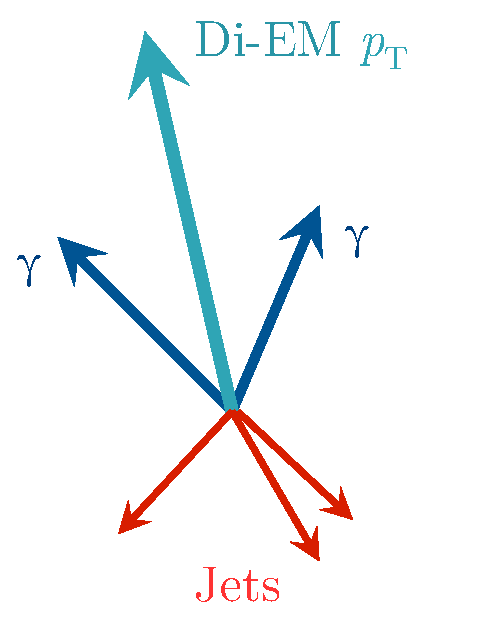
\includegraphics[width=0.3\textwidth]{Figures/DataAnalysis/Diempt.pdf}
\end{center}
\caption{The \diempt vector, shown in light blue, is the vector sum of the \pT of the two photons in the event, shown in blue. The magnitude of the \diempt vector is used to model the hadronic recoil, shown in red. }
\label{fig:diempt}
\end{figure*}

The \diempt distributions for the $\gamma\gamma$ candidate sample and the $ff$ control sample are shown in Figure~\ref{fig:ggffDiempt}. The $ff$ events are reweighted using the $\gamma\gamma$/$ff$ ratios displayed in the ratio plot of Figure~\ref{fig:ggffDiempt}. The $ff$ \ETmiss distribution is normalized to the \ETmiss $<~50$ GeV region of the $\gamma\gamma$ sample, where signal contamination is minimal. 

\begin{figure*}[h]
\begin{center}
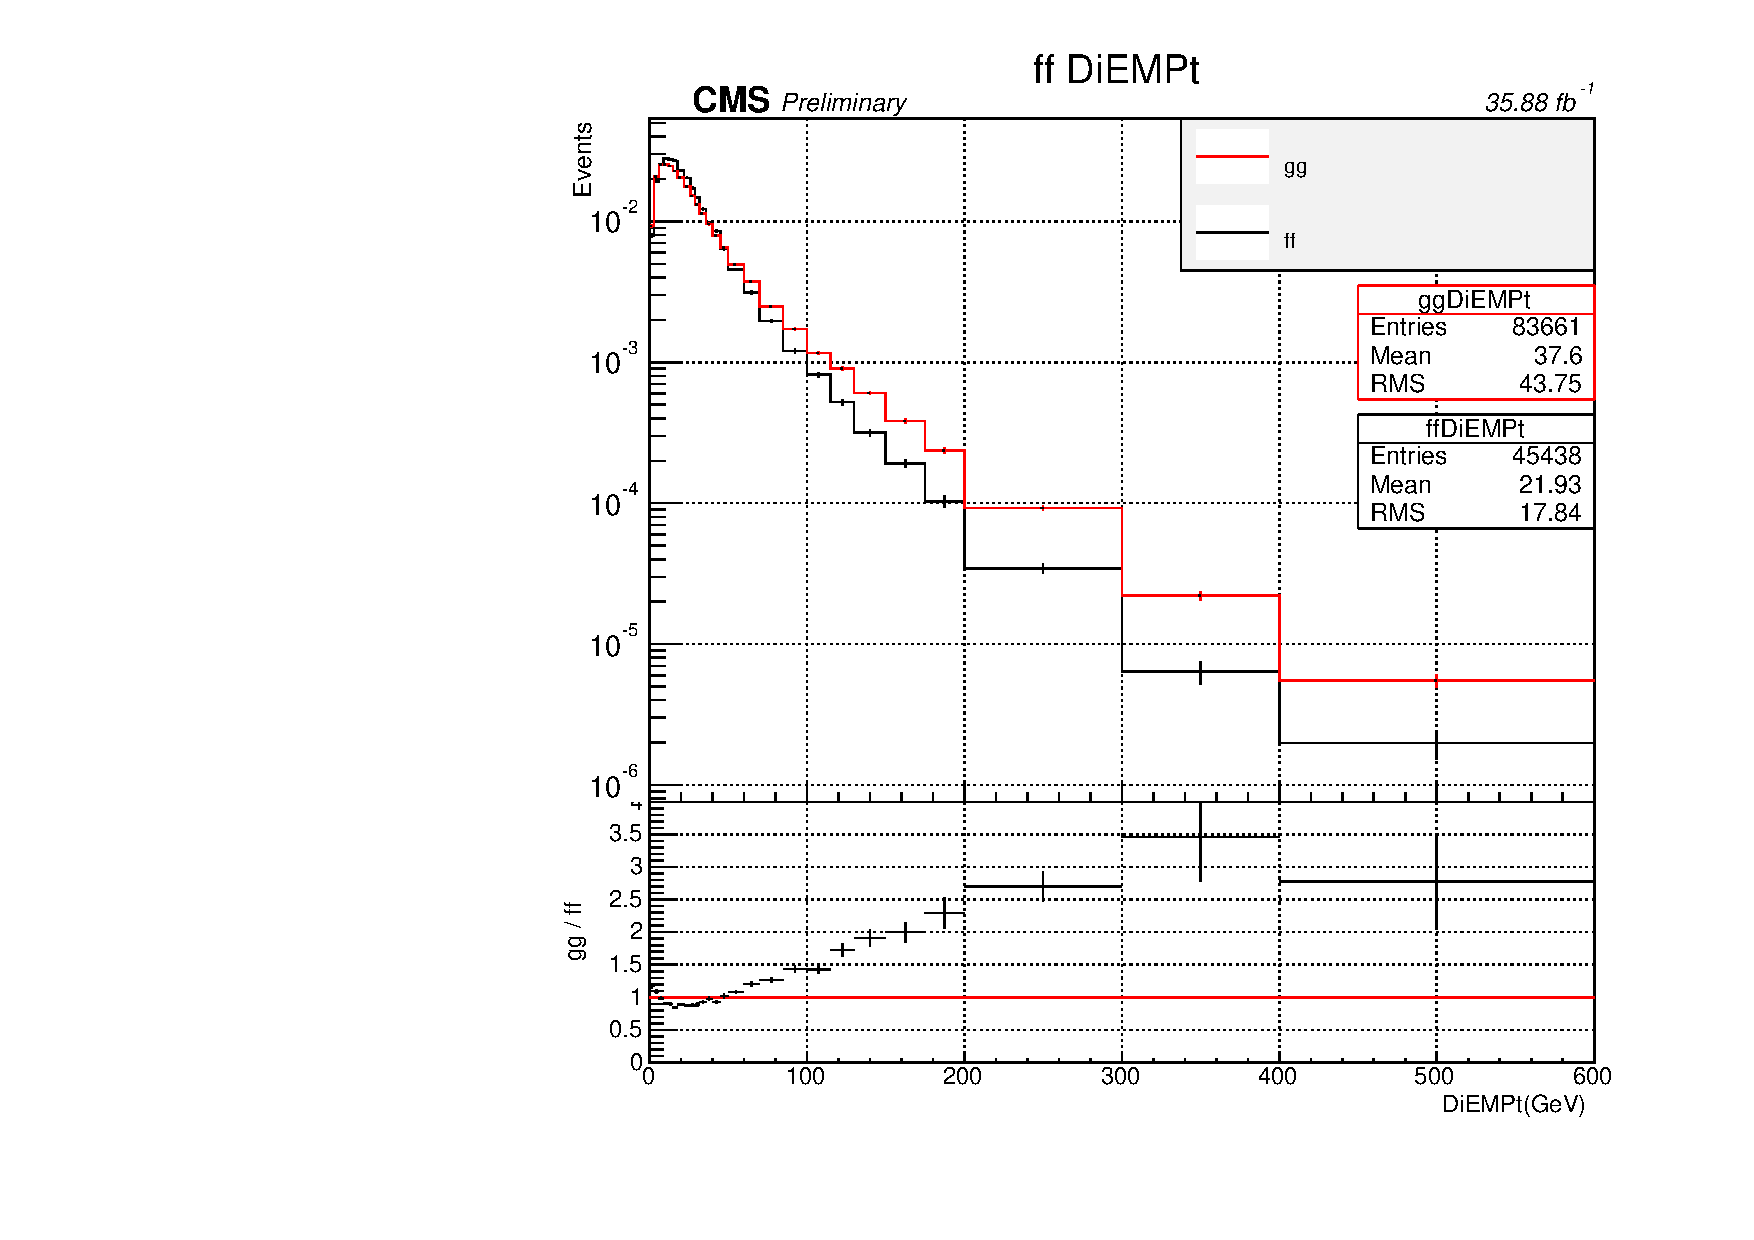
\includegraphics[width=0.9\textwidth]{Figures/DataAnalysis/ggffDiempt.pdf}
\end{center}
\caption{\Diempt distributions of the $ff$ control sample (black) and the $\gamma\gamma$ candidate sample (red). The ratio plot on the bottom shows the $\gamma\gamma$/$ff$ ratios that are used to reweight the $ff$ \ETmiss distribution. }
\label{fig:ggffDiempt}
\end{figure*}

The unweighted $ff$ and $\gamma\gamma$ \ETmiss distributions are shown in Figure~\ref{fig:ggffUnweighted}. A comparison between the unweighted and \diempt reweighted $ff$ \ETmiss distributions is shown in Figure~\ref{fig:compareUnweighted}. Finally, Figure~\ref{fig:ggffReweighted} compares the reweighted $ff$ \ETmiss distribution to the candidate $\gamma\gamma$ \ETmiss distribution.

\begin{figure*}[h]
\begin{center}
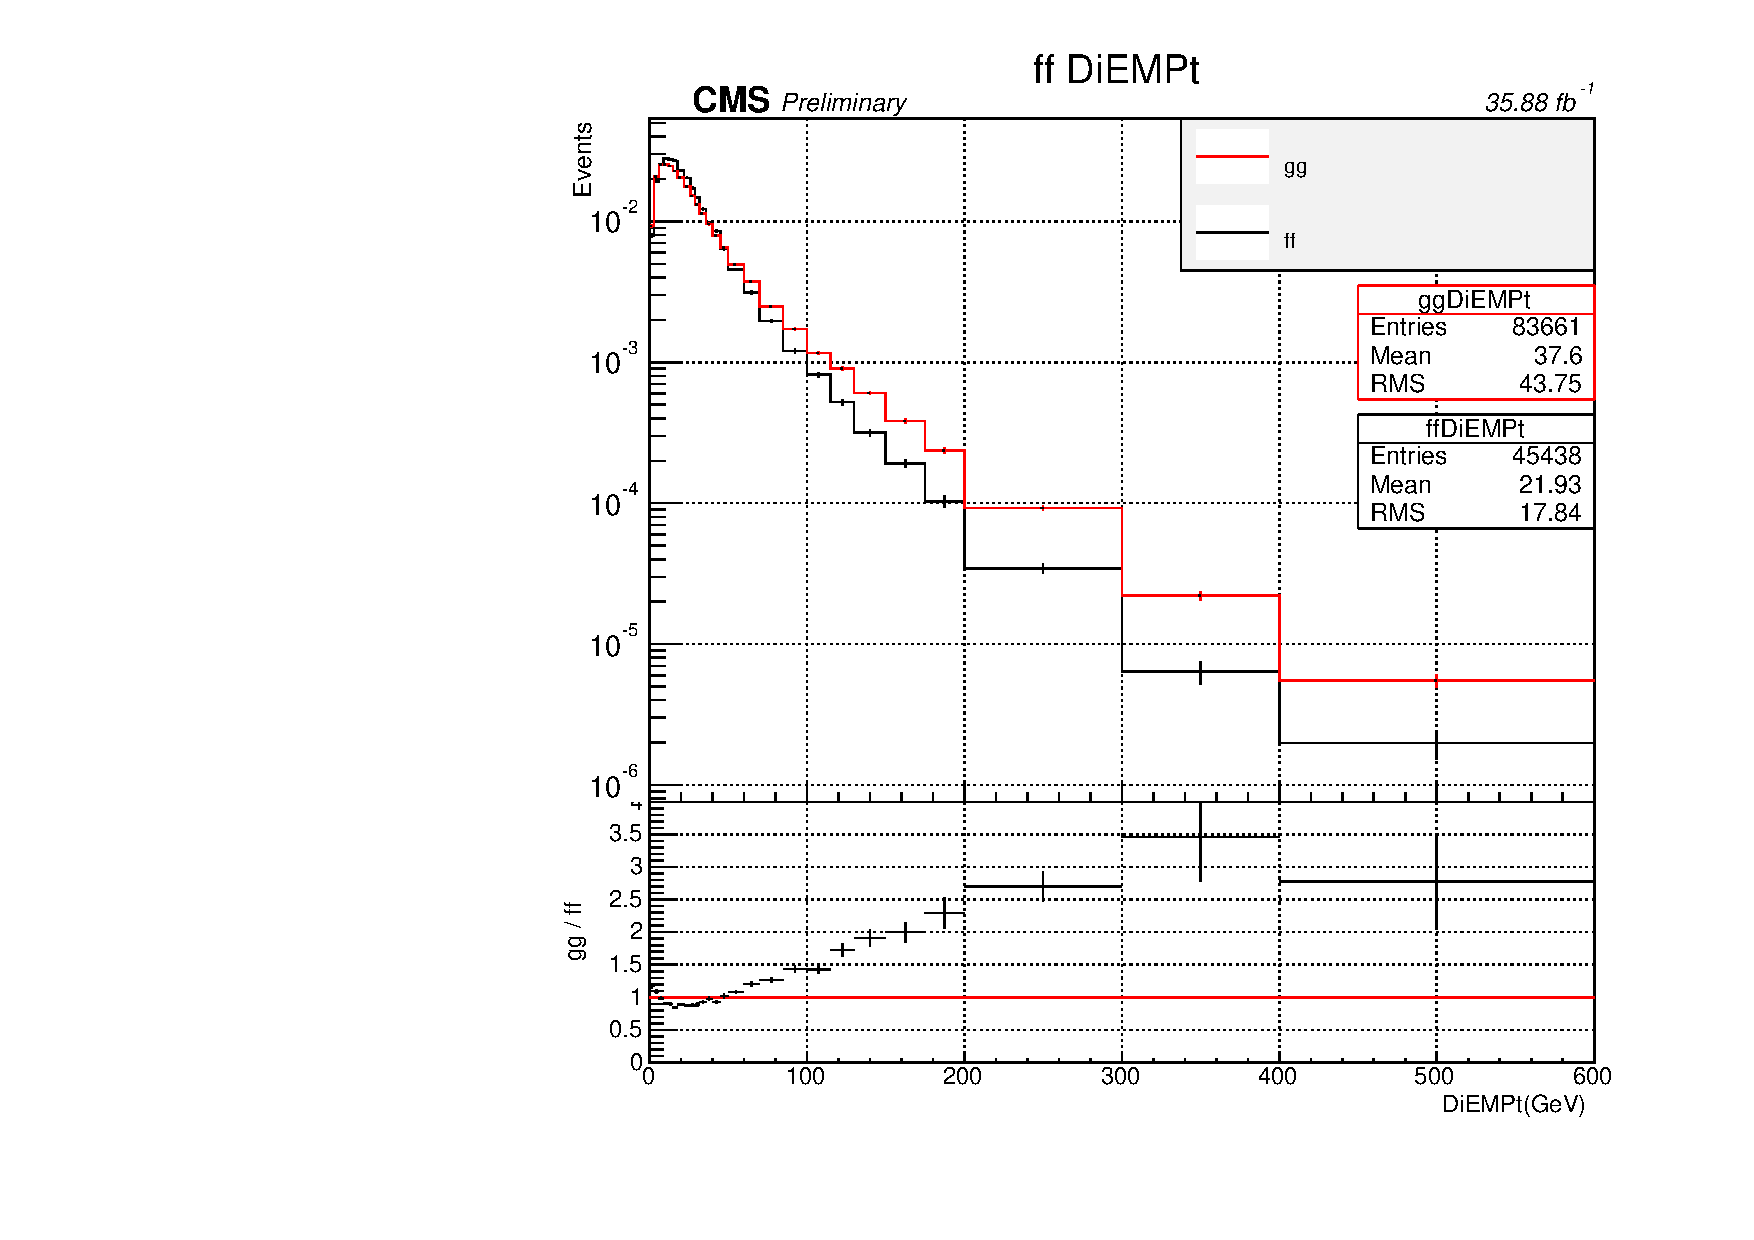
\includegraphics[width=0.9\textwidth]{Figures/DataAnalysis/ggffUnweighted.pdf}
\end{center}
\caption{\Diempt distributions of the $ff$ control sample (black) and the $\gamma\gamma$ candidate sample (red). The ratio plot on the bottom shows the $\gamma\gamma$/$ff$ ratios that are used to reweight the $ff$ \ETmiss distribution. }
\label{fig:ggffUnweighted}
\end{figure*}

\begin{figure*}[h]
\begin{center}
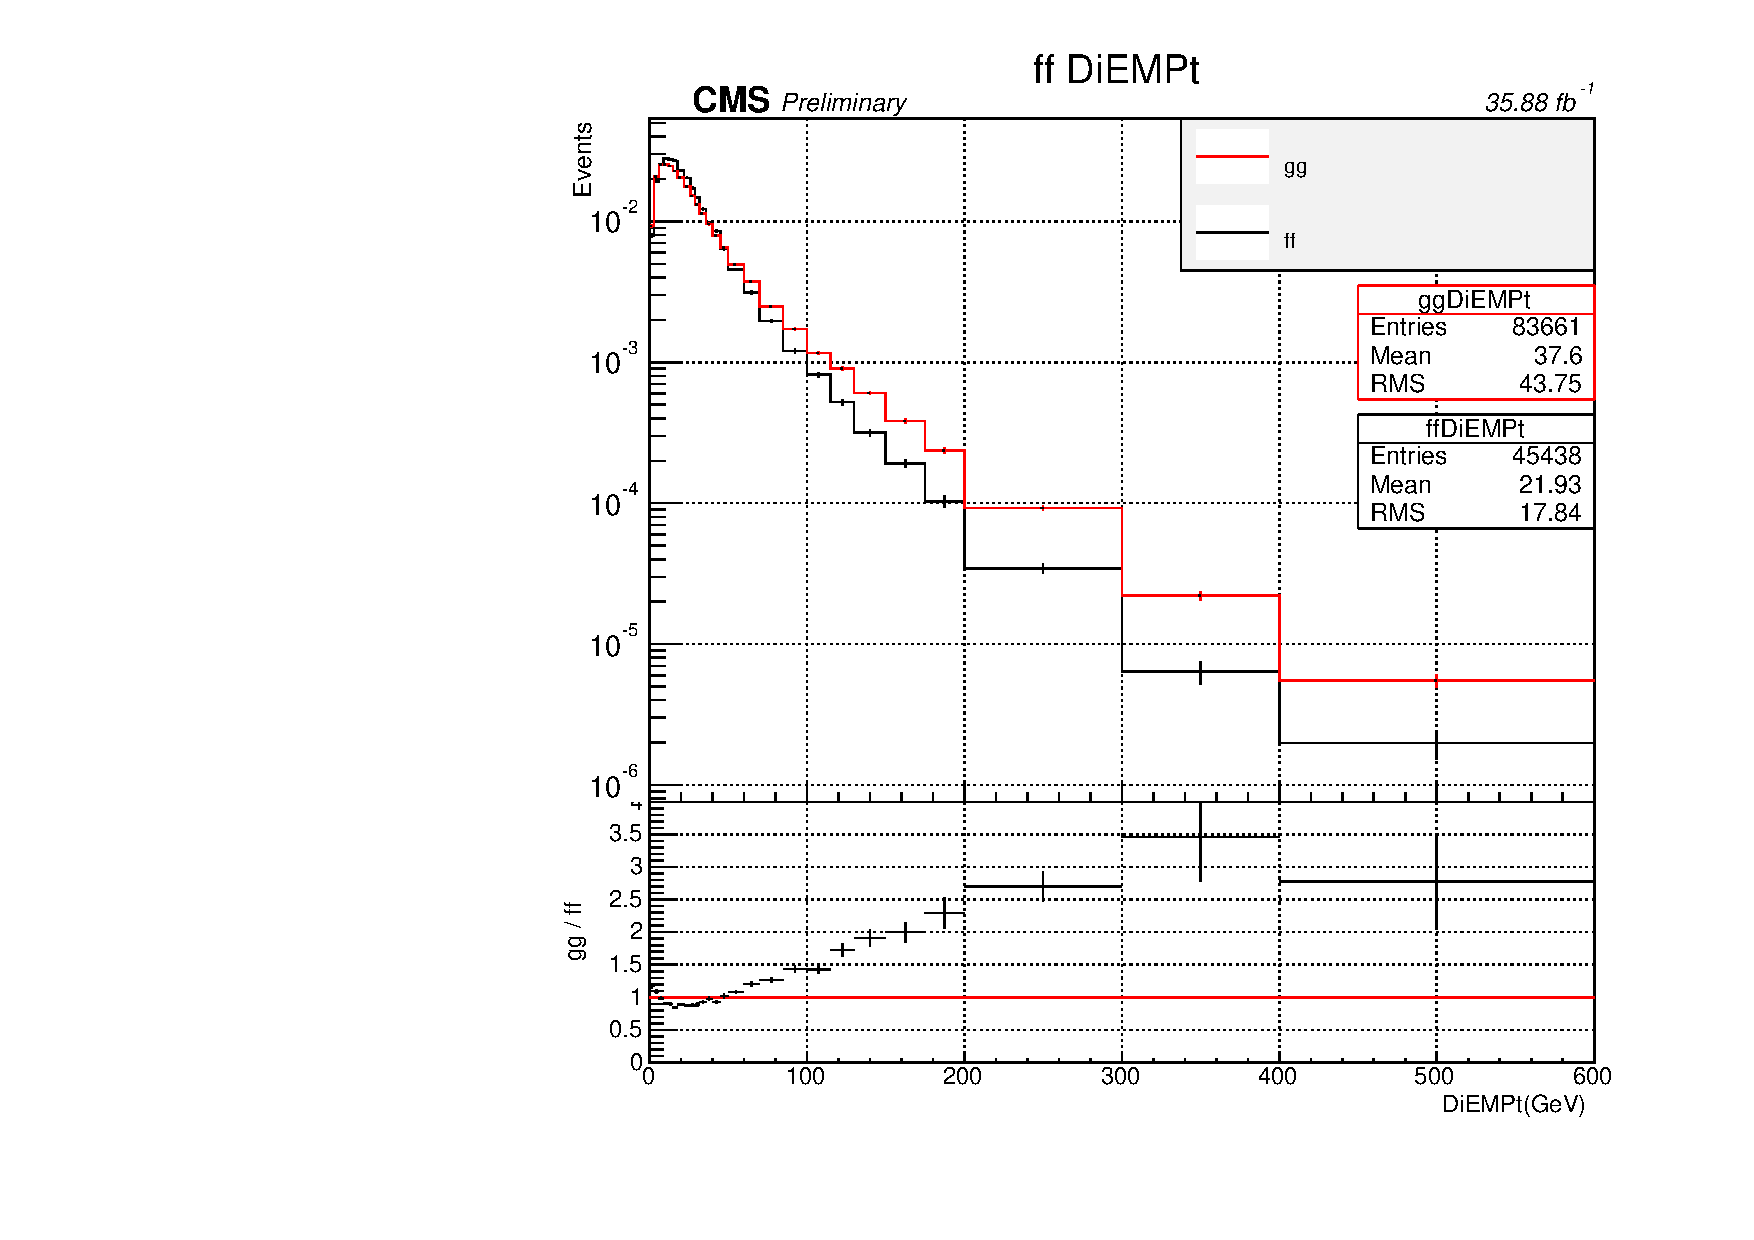
\includegraphics[width=0.9\textwidth]{Figures/DataAnalysis/compareUnweighted.pdf}
\end{center}
\caption{\Diempt distributions of the $ff$ control sample (black) and the $\gamma\gamma$ candidate sample (red). The ratio plot on the bottom shows the $\gamma\gamma$/$ff$ ratios that are used to reweight the $ff$ \ETmiss distribution. }
\label{fig:compareUnweighted}
\end{figure*}

\begin{figure*}[h]
\begin{center}
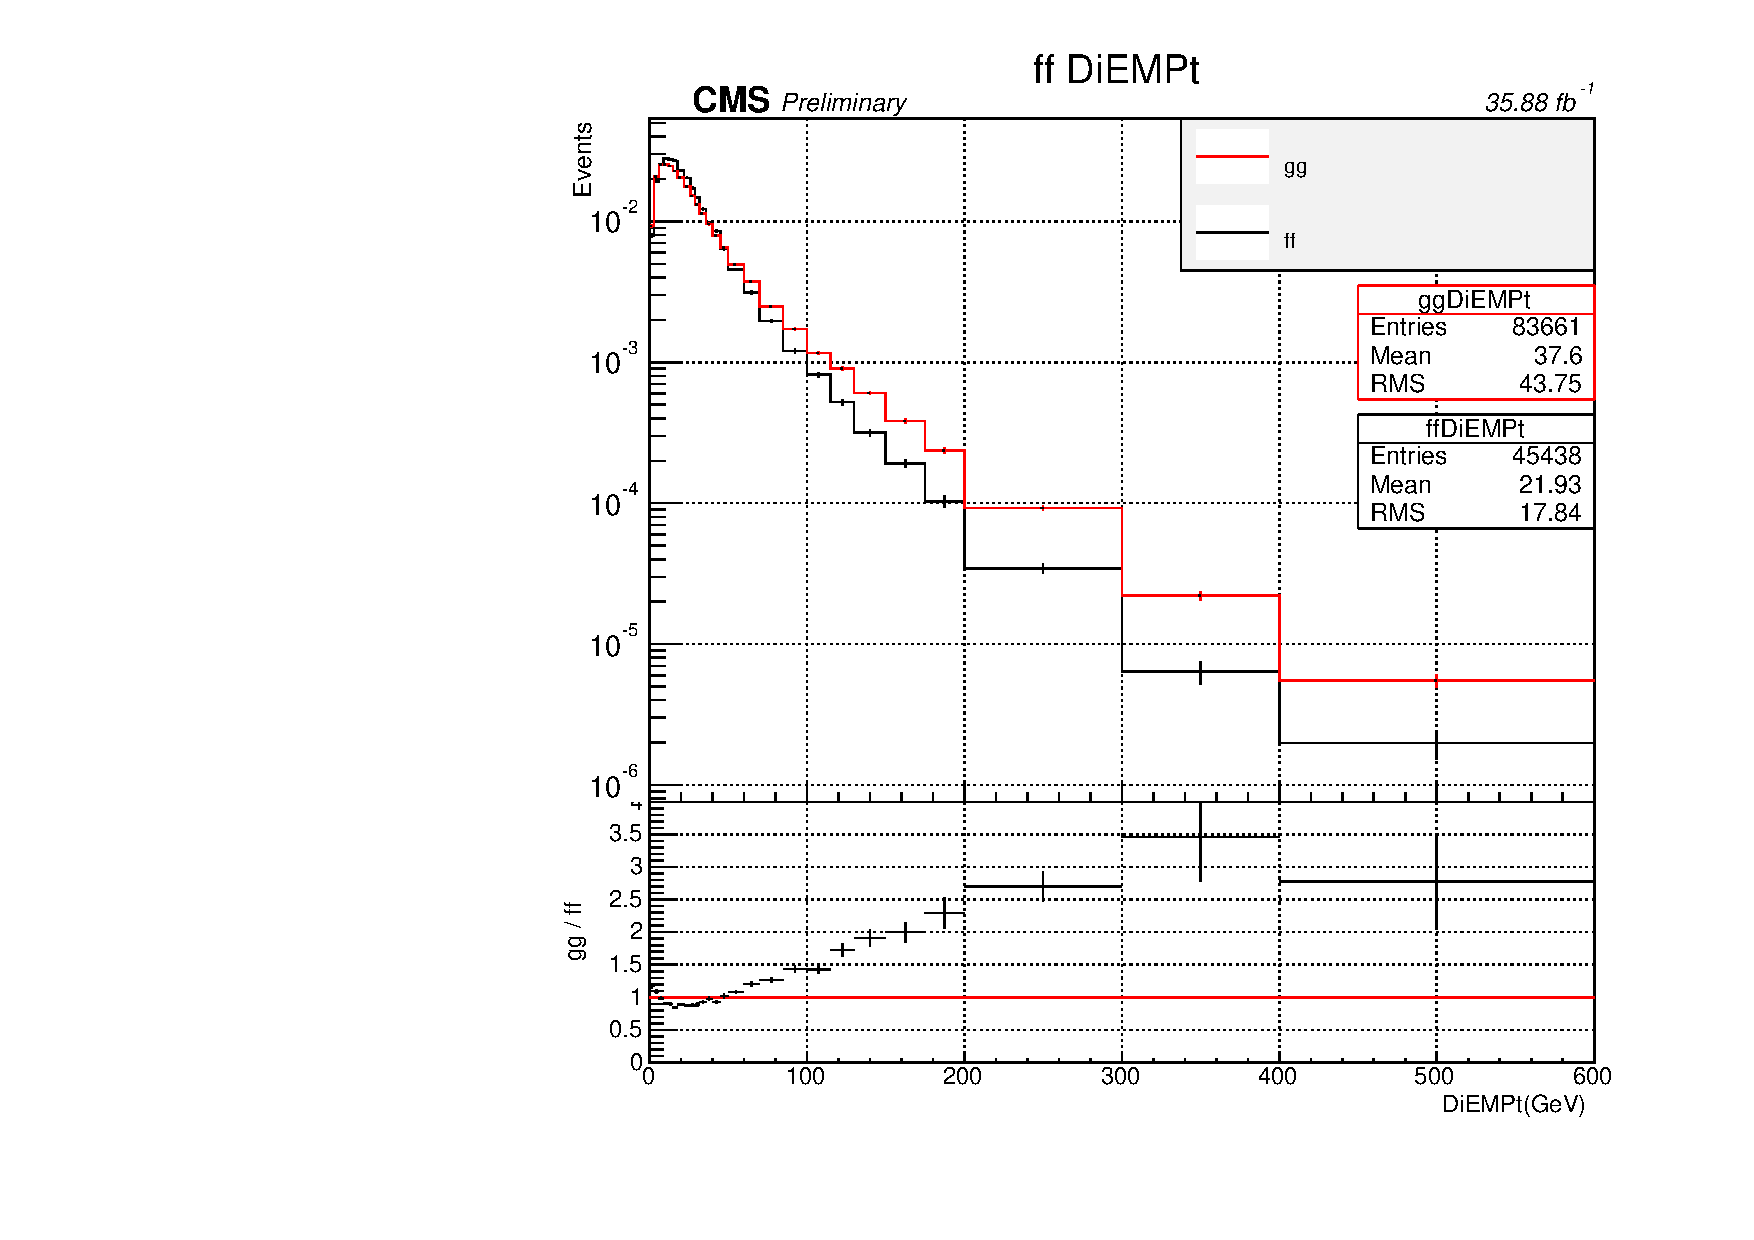
\includegraphics[width=0.9\textwidth]{Figures/DataAnalysis/ggffReweighted.pdf}
\end{center}
\caption{\Diempt distributions of the $ff$ control sample (black) and the $\gamma\gamma$ candidate sample (red). The ratio plot on the bottom shows the $\gamma\gamma$/$ff$ ratios that are used to reweight the $ff$ \ETmiss distribution. }
\label{fig:ggffReweighted}
\end{figure*}

%%%%%%Cross Check and Systematics%%%%%%

\subsection{Cross check on QCD background}
\label{sec:crossCheck}

In order to set a systematic uncertainty on the overall \ETmiss shape predicted using the \diempt reweighting method, we sought an alternate way to estimate the QCD background. This cross check relies on the assumption that the ratio of $\gamma\gamma$ events to $ff$ events should not depend sensitively on \ETmiss. If this assumption is true, then we should be able to extrapolate from the low-\ETmiss control region to the high-\ETmiss signal region.

\begin{figure*}[h]
\begin{center}
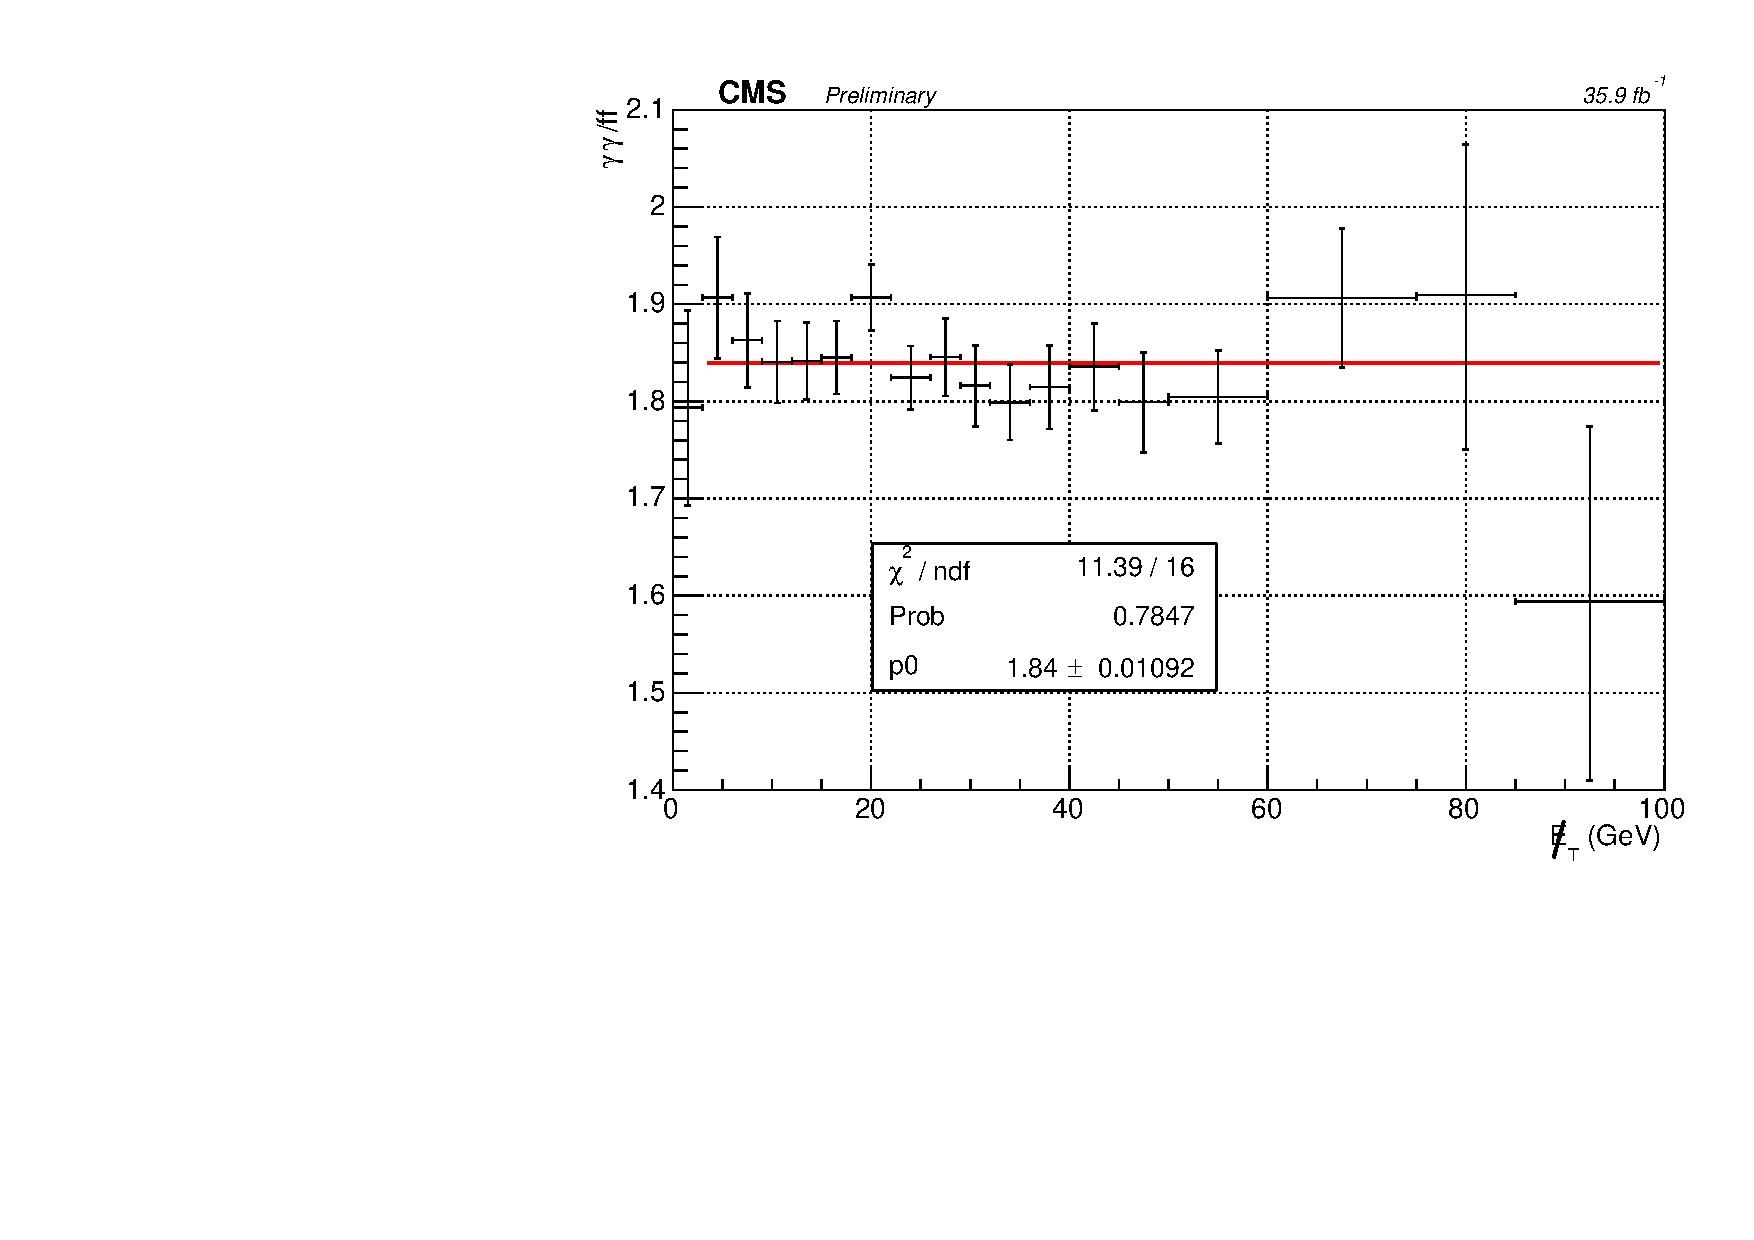
\includegraphics[width=0.9\textwidth]{Figures/DataAnalysis/crossCheckFit.pdf}
\end{center}
\caption{The ratio of $\gamma\gamma$ to $ff$ events for \ETmiss$ < 100$ GeV. 
The ratio has been fit to a constant function, which can then be used to 
extrapolate to the \ETmiss$ >100$ GeV signal region. 
This provides an alternative estimation method for the QCD background.}
\label{fig:crossCheck}
\end{figure*}

Figure~\ref{fig:crossCheck} shows the ratio of $\gamma\gamma$/$ff$ as a function of \ETmiss in the \ETmiss $<$ 100 GeV control region. The ratio has been fit to a constant function $f(\ETmiss)$. Using this function, the expected number of $\gamma\gamma$ events in bin $i$ of the signal region is given by the following equation:

\begin{equation}
N_{\gamma\gamma}^i = f(\ETmiss) \times N_{ff}^i 
\end{equation}

Table~\ref{tab:crossCheck} compares the expected QCD background contribution as predicted with the cross check method to that predicted with the \diempt reweighting method. For the cross check method, the uncertainty arising from the choice of fitting function is estimated by taking the difference between the results when fitting to a constant to the results when fitting to a linear function. In addition, the cross check uncertainties listed in Table~\ref{tab:crossCheck} include the statistical uncertainty from the limited control sample statistics and the $1~\sigma$ uncertainties from the fit. For the \diempt reweighting method, the uncertainties include the statistical uncertainty and the uncertainty from the \diempt reweighting procedure (this systematic is described in detail in Section~\ref{sec:QCDSysUncert}). 

\begin{table}[ht]
     \caption{COMPARISON BETWEEN REWEIGHTING METHOD AND RATIO METHOD FOR THE QCD BACKGROUND ESTIMATE}
     \centering
     {\renewcommand{\arraystretch}{1.2} %<- modify value to suit your needs                                                            
     \begin{tabular}{| c | c | c | c |}
     \hline
     \hline
    \ETmiss bin (Gev) & Reweighted ff estimate & Ratio method estimate \\
     \hline
    $100-115$ & ${69.23}^{+ 15.18}_{-12.68}$ & ${ 55.19}^{+ 12.03}_{-10.33}$ \\
    $115-130$ & ${30.89}^{+ 11.76}_{-8.82}$  & ${ 22.08}^{+ 8.39}_{-6.59}$ \\
    $130-150$ & ${25.98}^{+ 11.95}_{-8.61}$  & ${ 16.55}^{+ 7.56}_{-5.69}$ \\
    $150-185$ & ${20.49}^{+ 10.12}_{-7.11}$  & ${ 14.72}^{+ 7.26}_{-5.45}$ \\
    $185-250$ & ${8.74}^{+ 11.65}_{-5.89}$   & ${ 3.68}^{+ 4.85}_{-2.47}$ \\
    $> 250$     & ${5.13}^{+ 11.86}_{-4.43}$   & ${ 1.84}^{+ 4.23}_{-1.60}$ \\
     \hline
     \hline
     \end{tabular}
}
	\justify{Comparison of the background estimate using the di-EM \pt reweighting method and the $\gamma\gamma$/$ff$ ratio method. The uncertainties on the 
	 di-EM \pt reweighting method include the statistical uncertainties and the reweighting uncertainty. The uncertainties on the ratio method include the 
	 statistical uncertainties, the uncertainties in the fit parameter, and the uncertainty from the choice of fit function. }
     \label{tab:crossCheck}
\end{table}


The two methods give overlapping predictions
within uncertainty, and therefore this cross check serves to validate our di-EM \pt reweighting
background estimation method. The difference between the two methods
is taken as a systematic uncertainty on the overall \ETmiss shape.

%%%%%%%%%%%%%%%%%%%%%%%%%%%%%%%%%%%%%%%
%%%%%%%%EWK background %%%%%%%%%%%%%%%%%%%%%%
%%%%%%%%%%%%%%%%%%%%%%%%%%%%%%%%%%%%%%%

\section{Electroweak background}
\label{sec:EWK}

The subdominant background for this search is comprised of W$\gamma$ and W+jet events where W$\rightarrow e \nu$ and the electron is misidentified as a photon. This background is referred to as the electroweak (EWK) background. Unlike the QCD background, there is inherent \ETmiss in these events from the escaping neutrino. 

To estimate this background, we first calculate the rate at which electrons are misidentified as photons. This is done by comparing the invariant mass peak in a double electron sample ($ee$) with the invariant mass peak in a sample of events with one electron and one photon ($e\gamma$). The composition of the $e\gamma$ control sample is investigated in Section~\ref{sec:EWKMC} and the calculation of this ``fake rate" is described in detail in Section~\ref{sec:fakeRate}. To get the final expected contribution from the EWK background in our signal region, the fake rate is used to calculate a transfer factor (Section~\ref{sec:transfer}). By applying the transfer factor to an $e\gamma$ control sample, we are able to estimate how many of our candidate $\gamma\gamma$ events are actually events with one photon and one electron that has been misidentified as a photon (Section~\ref{sec:EWKresults}). 

%%%%%%%%%%%%%%%%%%%%%%%%%%%%%%%%%%%%%%%

\subsection{Composition of $e\gamma$ sample}
\label{sec:EWKMC}
The $e\gamma$ control sample is primarily made up of $\gamma~+$ jets or W$\gamma$ events. A data versus MC comparison of this control sample is shown in Figure~\ref{fig:dataMCEG}. The data distribution was fit using the simulated $\gamma~+$ jet and W$\gamma$ shapes as templates. From the fit, it was determined that 80\% of the $e\gamma$ events observed in data are from $\gamma~+$ jets  processes, and the remaining 20\% are W$\gamma$ events.  
In the \ETmiss$>100$~GeV signal region, however, W$\gamma$ events dominate.
For $100 < \ETmiss < 130$~GeV, 12.1\% of the MC prediction is made up of
$\gamma~+$ jet processes. For $\ETmiss >130$~GeV, 
$\gamma~+$ jet events contribute only 2.6\%.

\begin{figure*}[h!]
	\centering
	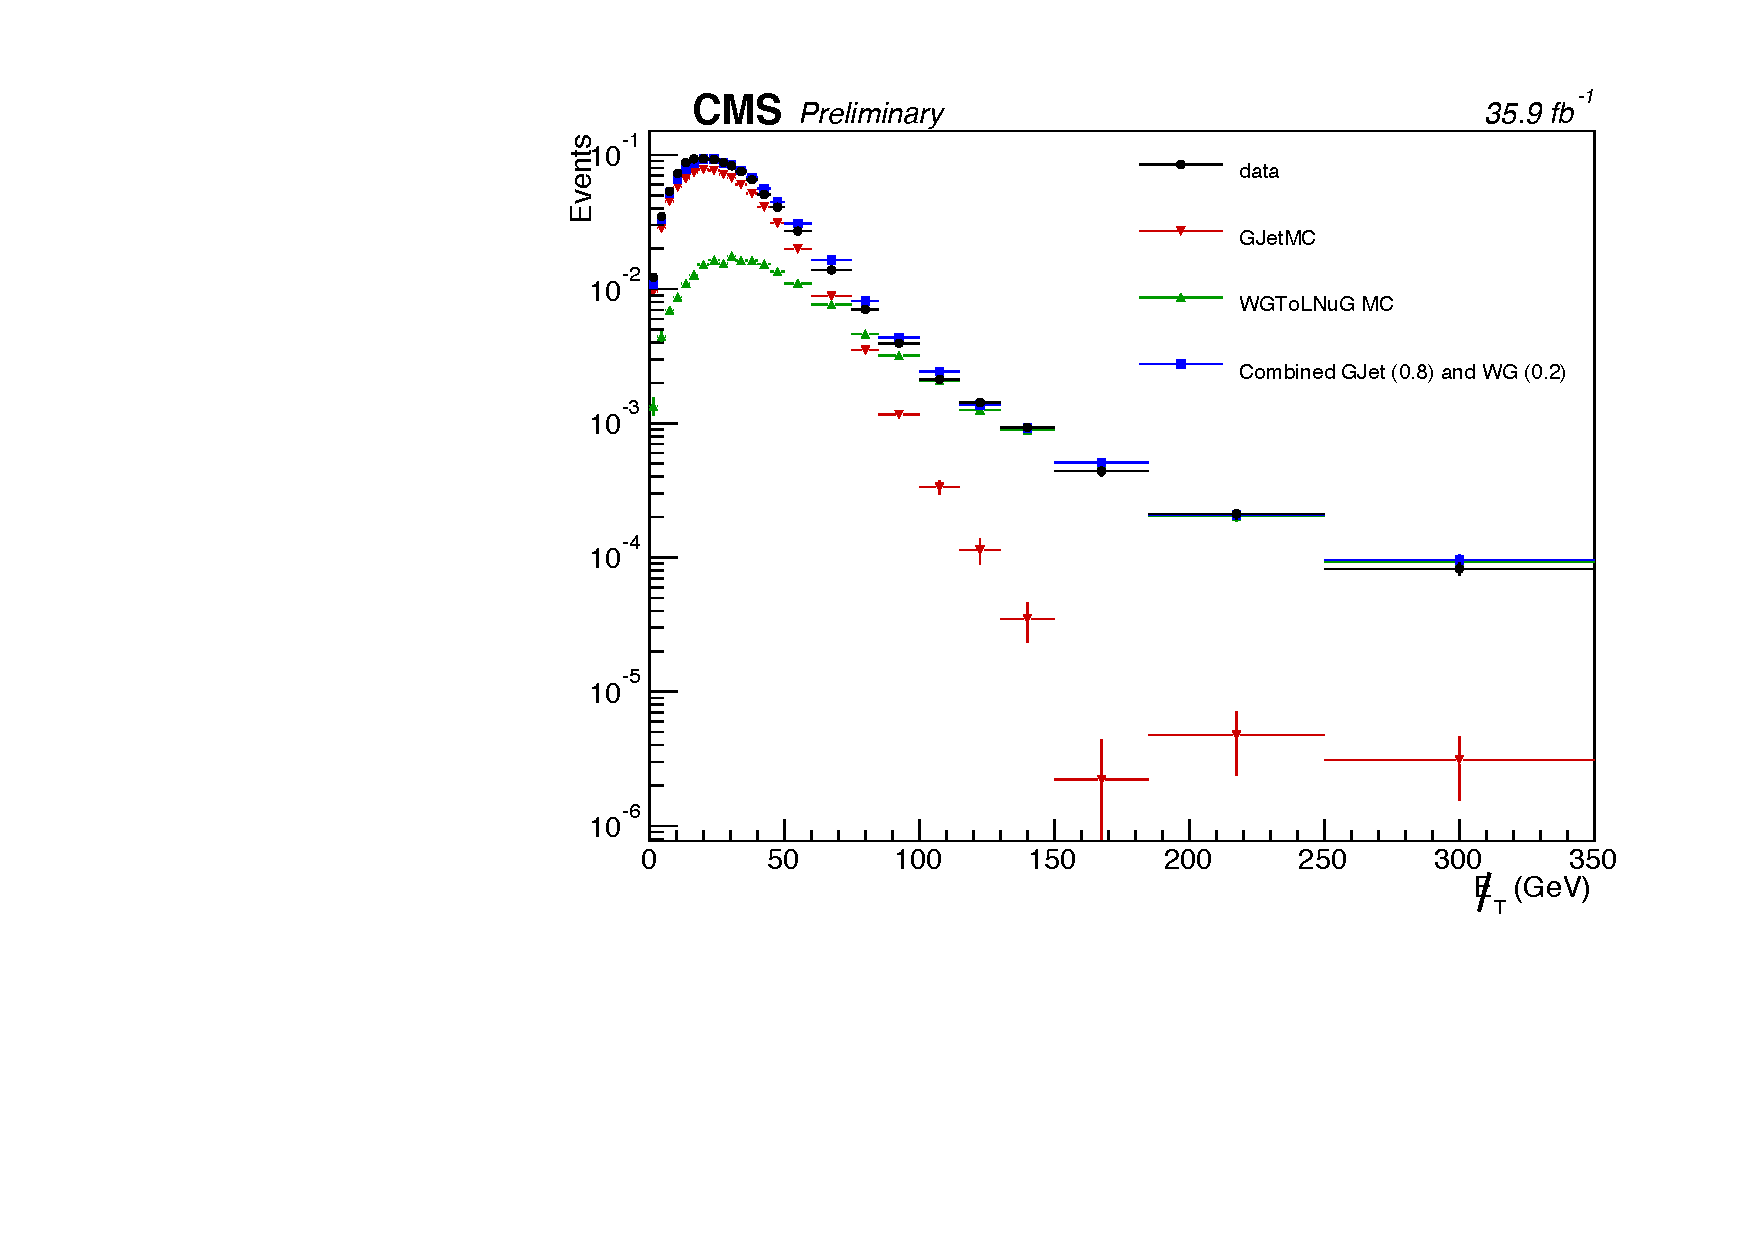
\includegraphics[width=0.8\textwidth]{Figures/DataAnalysis/dataMC_EG.pdf}
       \caption{Data versus MC comparison of the $e\gamma$ control sample \ETmiss distribution. To determine the relative contributions of the
       $\gamma~+$ jet and W$\gamma$ processes, the data distribution was fit using the $\gamma~+$ jet and W$\gamma$ shapes as templates. The data
       are shown in black, and the total MC prediction is shown in blue. The $\gamma~+$ jet MC (red) was scaled to 80\% of the observed events in data. and 
       the W$\gamma$ MC (green) was scaled to 20\% of the data distribution.
	}
   	\label{fig:dataMCEG}
\end{figure*}

%%%%%%%%%%%%%%%%%%%%%%%%%%%%%%%%%%%%%%%

\subsection{Fake rate calculation}
\label{sec:fakeRate}

A tag and probe method is used for the fake rate calculation. Events are selected using a single electron trigger. Electrons passing medium ID criteria and 
satisfying \pT $> 30$ GeV and $|\eta| < 2.1$ are used as tags. The tags are required to be matched to the object firing the single electron trigger within \dR$ < 0.2$. 
Probes are photon candidates with \pT $> 40$ GeV that pass all of the identification criteria described in Chapter~\ref{chap:EventSelect} except for the pixel seed veto. The tag and probe objects are required to be separated by \dR$ > 0.3$ and have an invariant mass between 40 and 140 GeV. If there are multiple tag and probe pairs in a single event, all possible combinations are considered. If the probe has a pixel seed, then it is labeled as an electron and falls into the $ee$ sample. If the probe does not have a pixel seed, however, then it is labeled as a photon and is included in the $e\gamma$ sample. 

Because processes other than $Z\rightarrow ee$ decays can be included in this sample, a fit is performed on each invariant mass distribution. The shape of the invariant mass peak in $Z\rightarrow ee$ MC is used as a signal template, and an electron + muon control region in data is used as the background template. After fitting the $ee$ and $e\gamma$ distributions in data, the integrals of the signal shapes between 80 and 100 GeV are referred to as $N_{ee}^Z$ and $N_{e\gamma}^Z$, respectively. 
Figure~\ref{fig:invMassShapes} shows the shapes of the data distributions as well as the background and signal templates with arbitrary normalization. The results after the fit are shown as well. 

\begin{figure*}[h]
\begin{center}
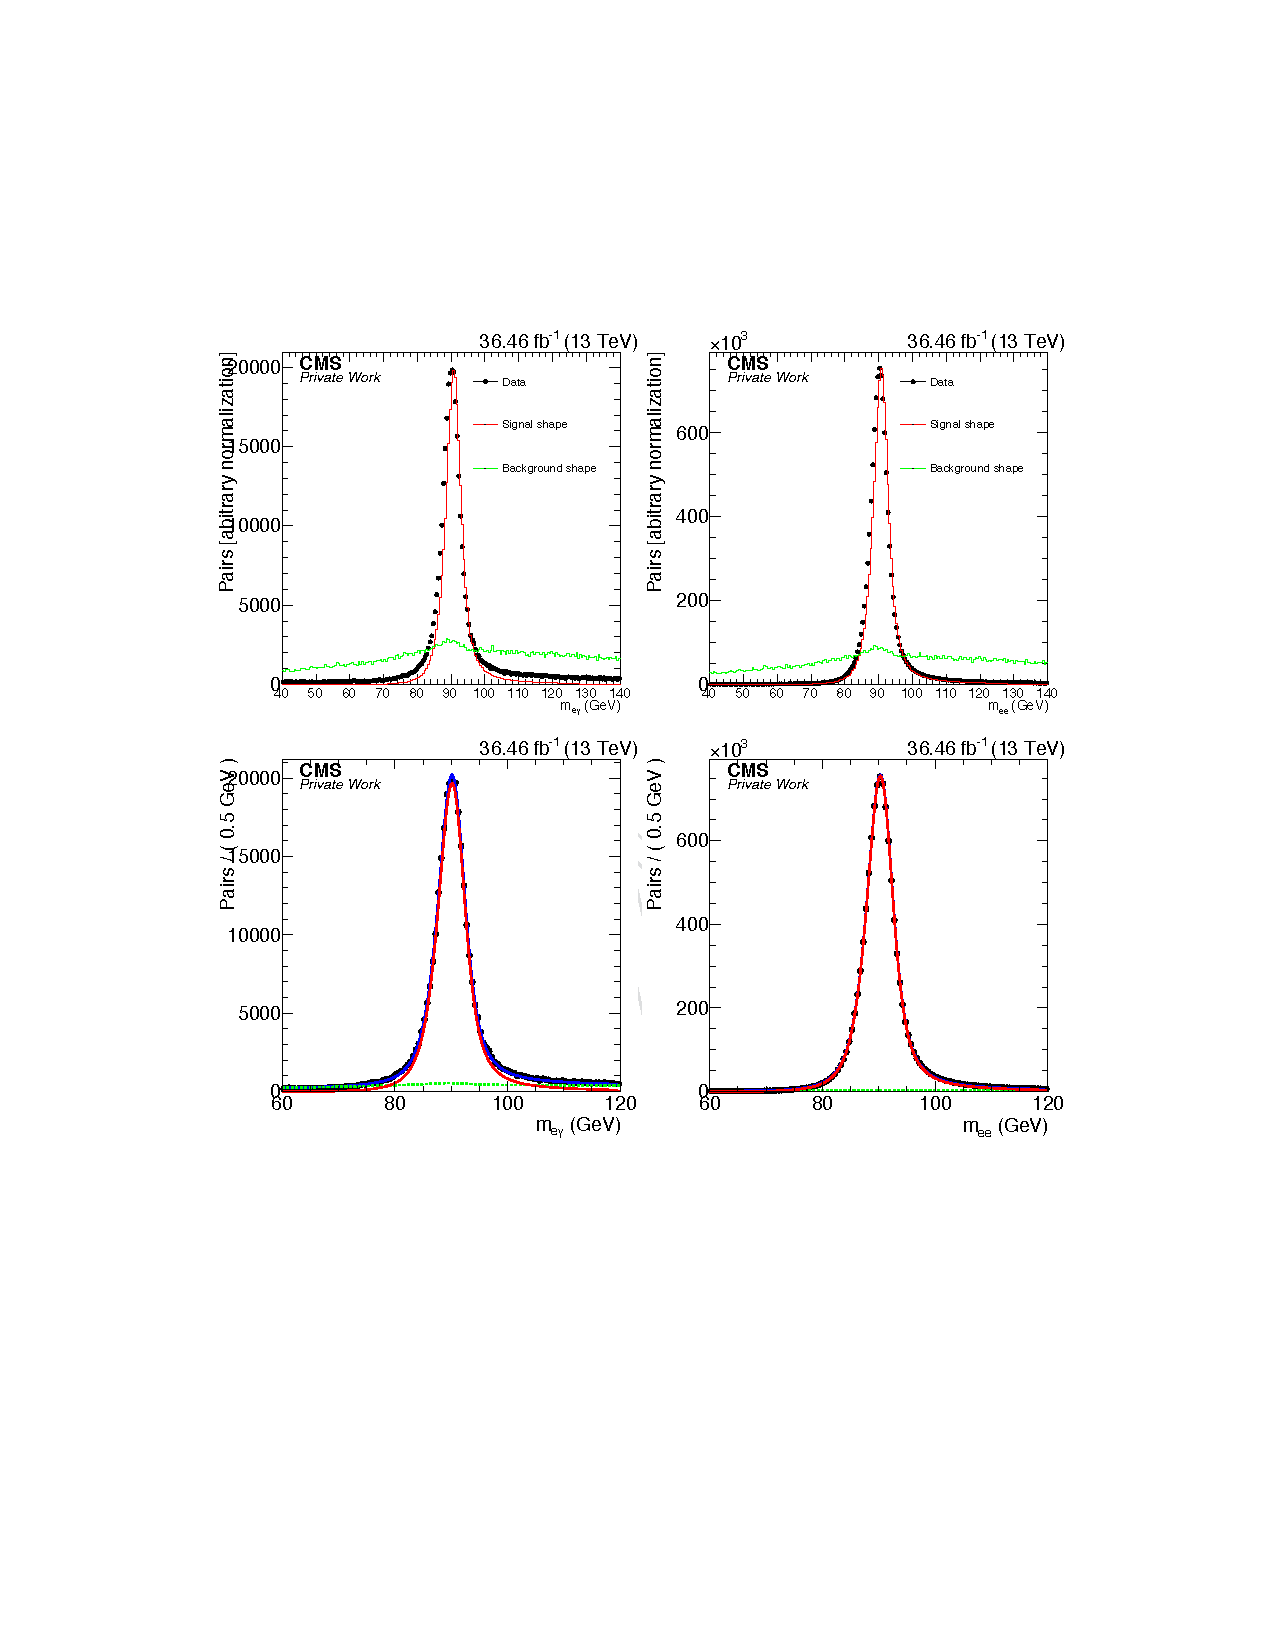
\includegraphics[width=\textwidth]{Figures/DataAnalysis/EWKInvMassShapes.pdf}
\end{center}
\caption{Invariant mass distributions for the $e\gamma$ (left) and $ee$ (right) samples. Each plot includes the data (black markers), 
the signal template (red), and the background template (green). The top plots demonstrate the shape of each distribution with arbitrary 
normalization, and the bottom plots show the distributions after the fits are performed.
}
\label{fig:invMassShapes}
\end{figure*}

The maximum of the background shape at 90 GeV arises from the \pT thresholds of the tag and probe objects. The \pT distributions tend to be sharply falling, so most probes have a \pT around 40 GeV and most tags have a \pT around 30 GeV. Changing the probe \pT threshold changes the position of the peak in the background template.

The ratio $R_{\gamma/e} = N_{e\gamma}^Z/N_{ee}^Z$ is calculated from the fits and found to be $R_{\gamma/e} = 2.63\%$ overall. The fits are performed in bins of different kinematic variables to investigate any potential dependencies of $R_{\gamma/e}$. These are shown in Figures~\ref{fig:fakeRateKin1} and \ref{fig:fakeRateKin2}. 

\begin{figure*}[h]
\begin{center}
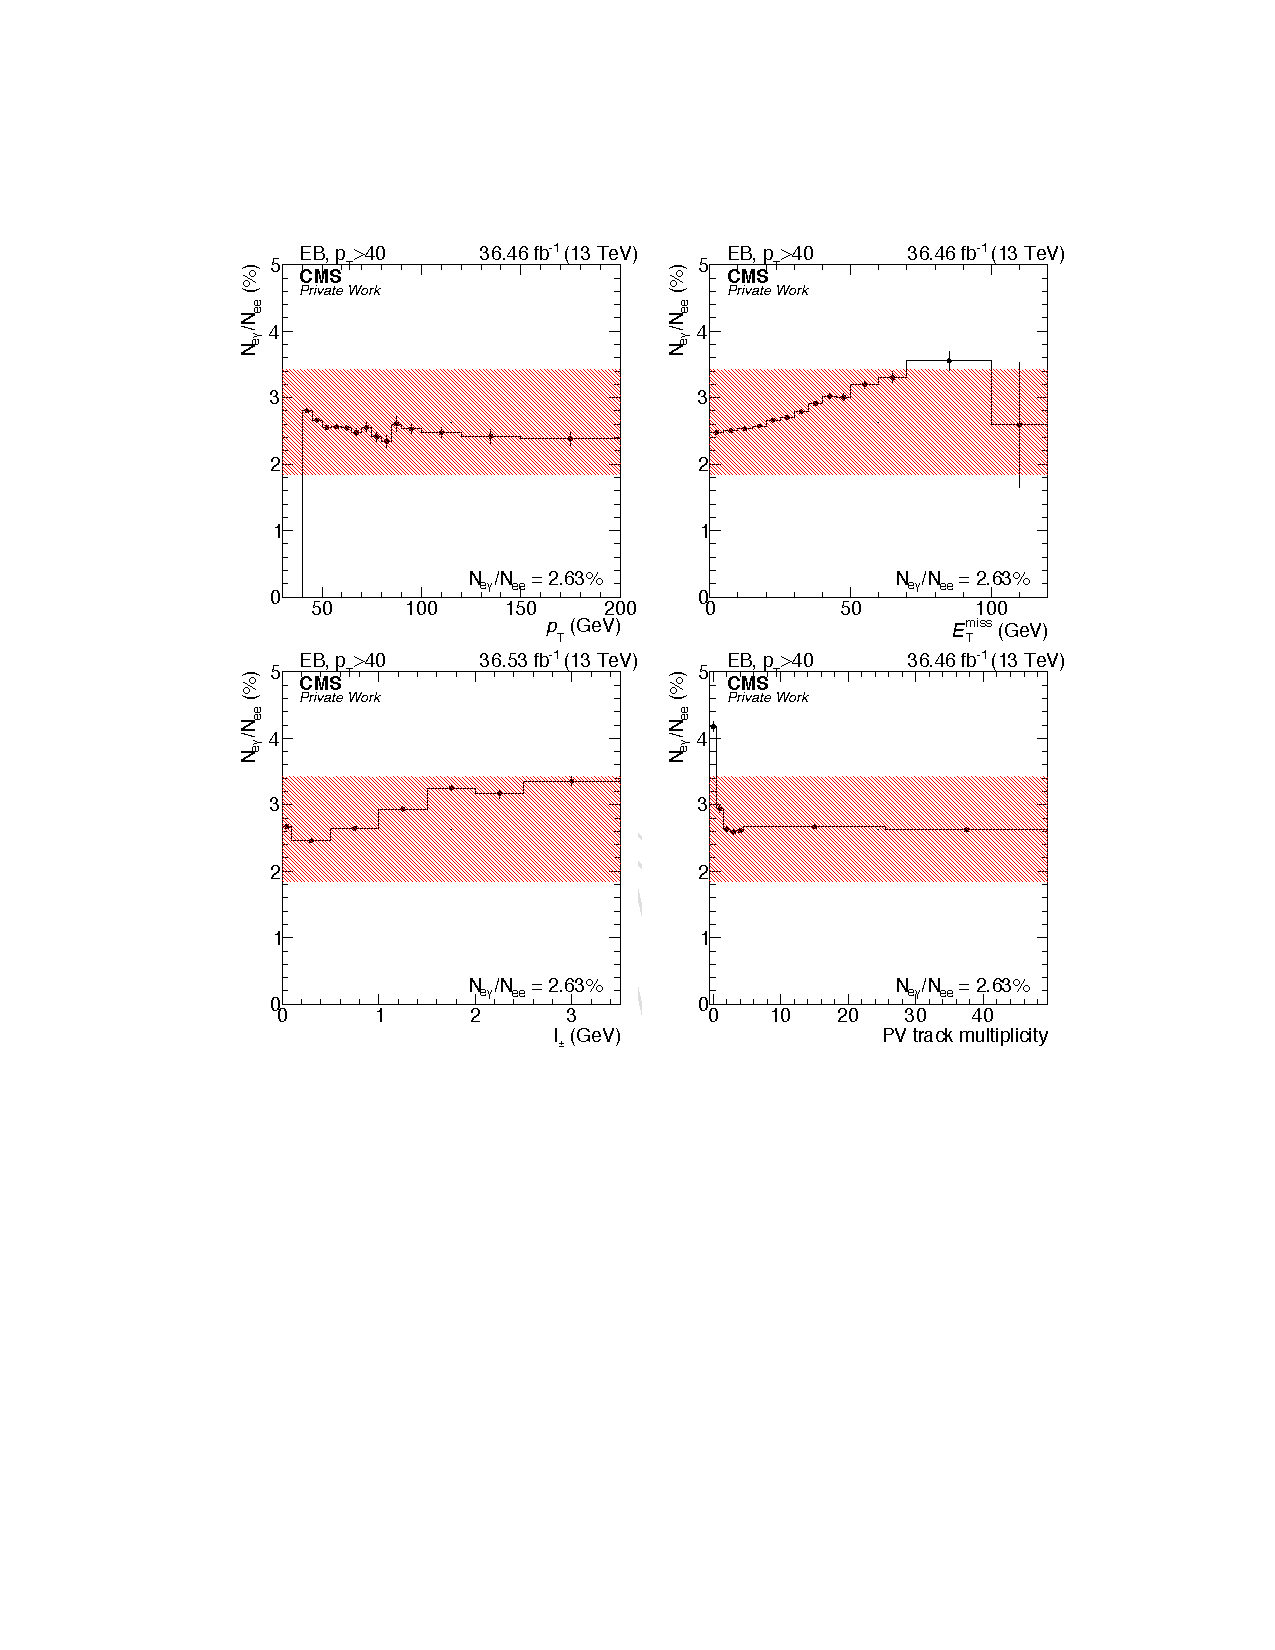
\includegraphics[width=\textwidth]{Figures/DataAnalysis/fakeKin1.pdf}
\end{center}
\caption{Value of $R_{\gamma/e}$ as a function of various kinematic variables for probes in the barrel: probe \pT, \ETmiss, isolation I$_{\pm}$, 
and track multiplicity of the primary vertex (PV). The red band corresponds to a 30\% uncertainty 
on $R_{\gamma/e}$.
}
\label{fig:fakeRateKin1}
\end{figure*}

\begin{figure*}[h]
\begin{center}
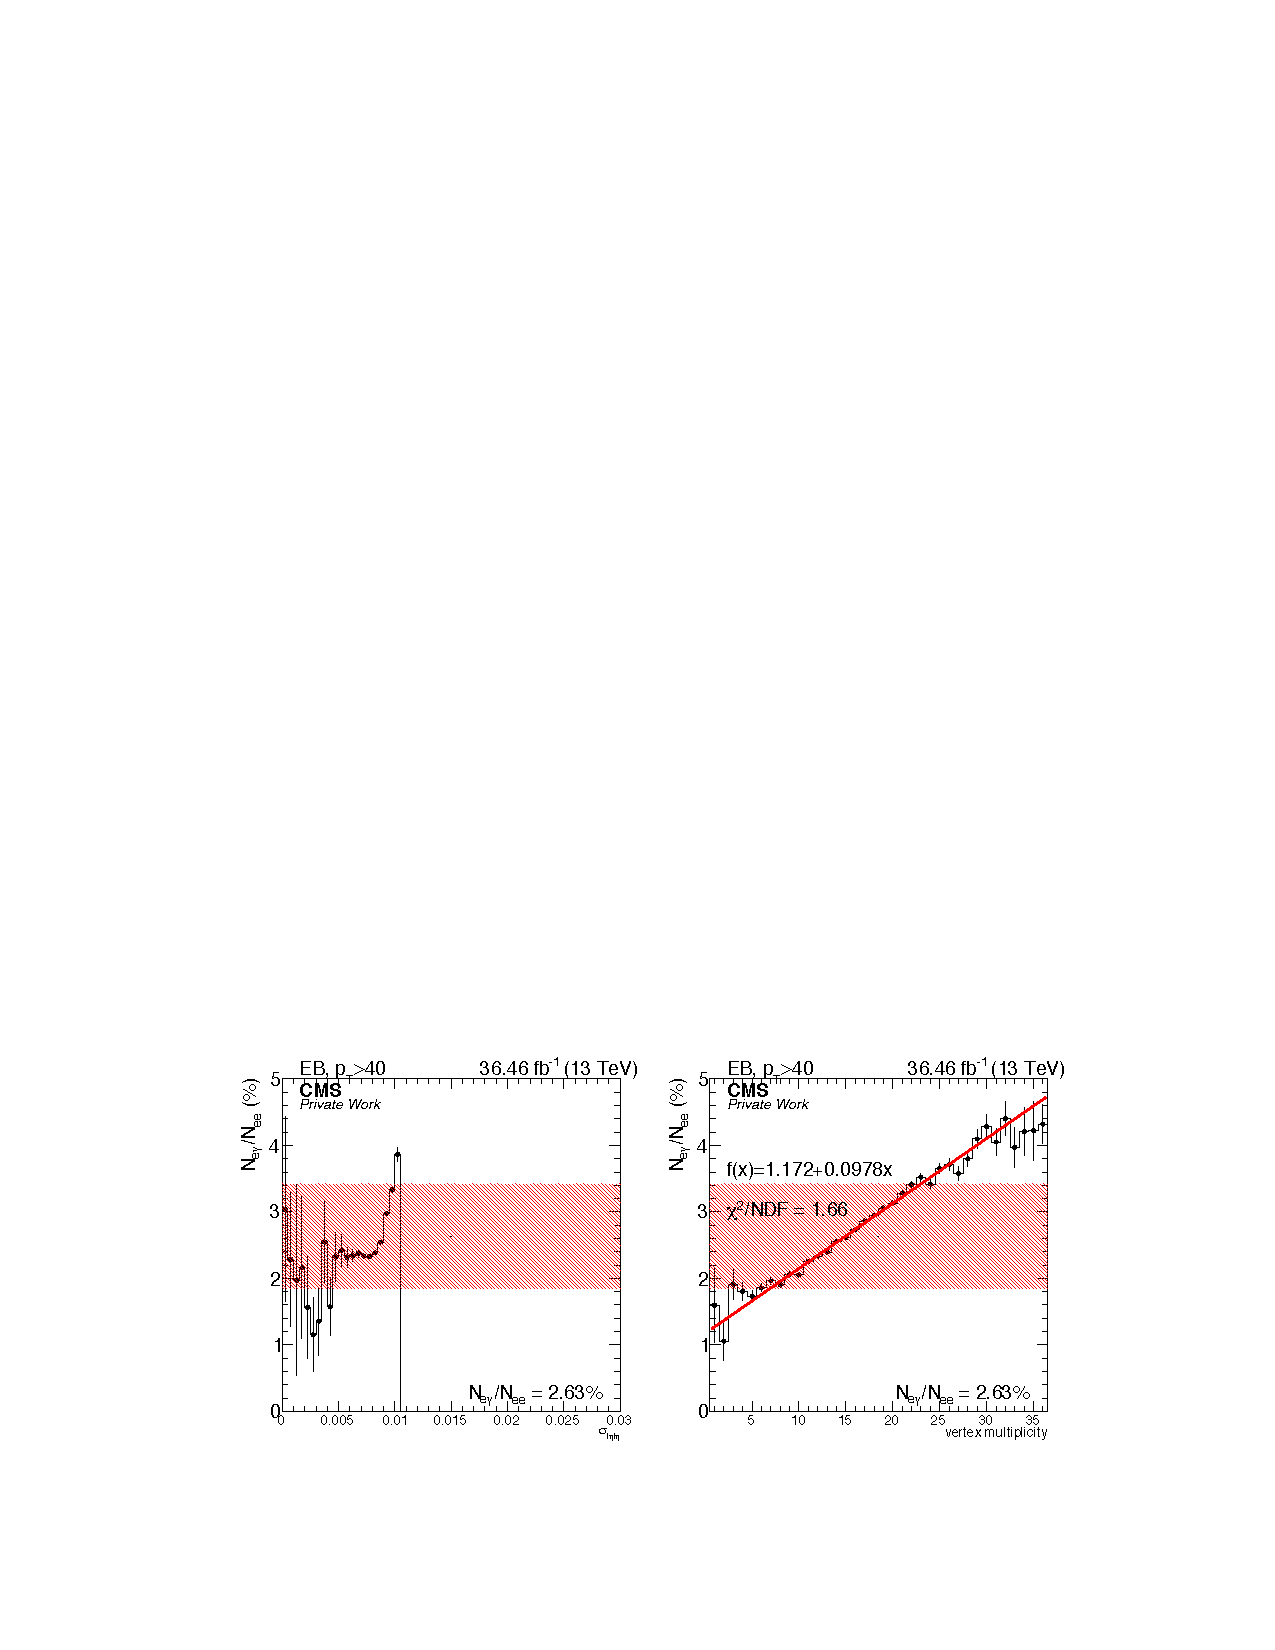
\includegraphics[width=\textwidth]{Figures/DataAnalysis/fakeKin3.pdf}
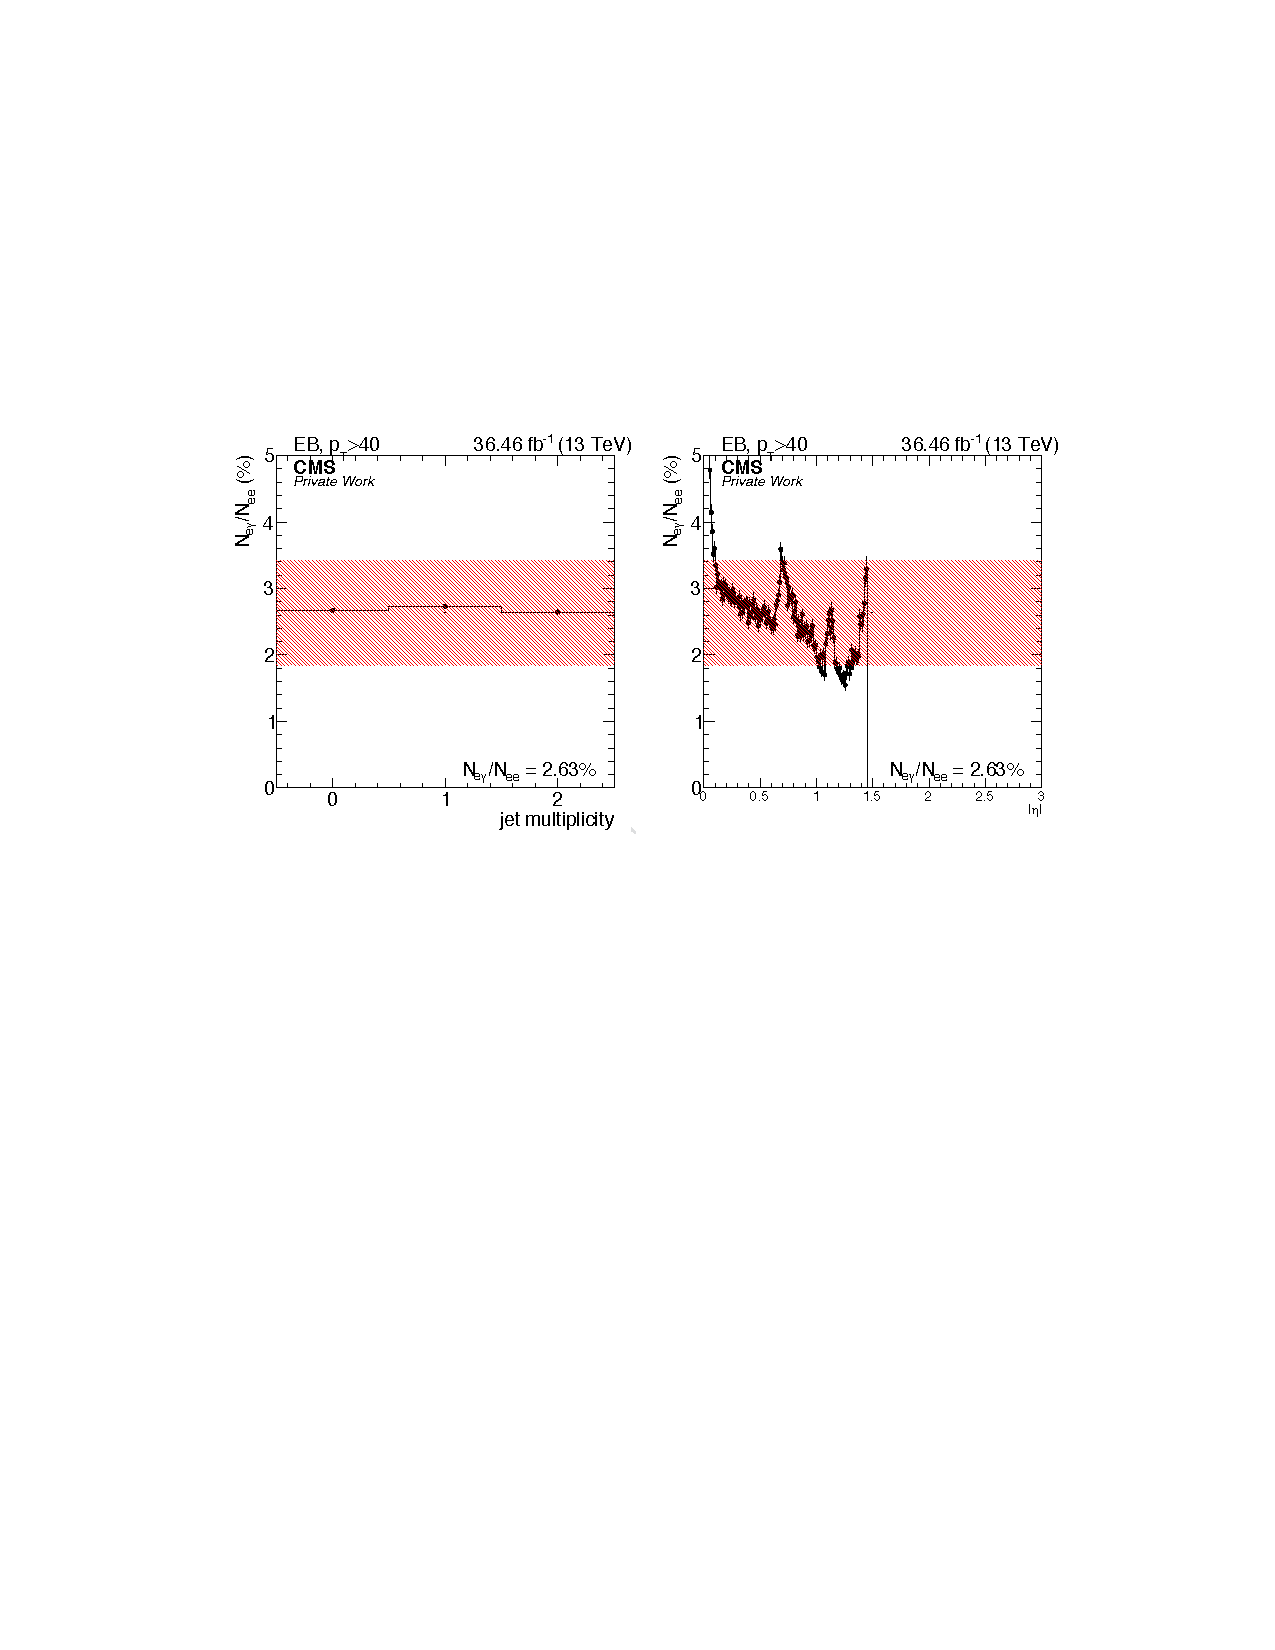
\includegraphics[width=\textwidth]{Figures/DataAnalysis/fakeKin2.pdf}
\end{center}
\caption{Value of $R_{\gamma/e}$ as a function of various kinematic variables for probes in the barrel: \sigmaietaieta of the probe, 
vertex multiplicity, jet multiplicity, and probe $|\eta|$. The red band corresponds to a 30\% uncertainty 
on $R_{\gamma/e}$.
}
\label{fig:fakeRateKin2}
\end{figure*}

A 30\% systematic uncertainty is assigned to the ratio $R_{\gamma/e}$ to cover the observed dependencies. 
This is shown in the red bands in Figures~\ref{fig:fakeRateKin1} and \ref{fig:fakeRateKin2}. The strongest dependency is with respect
to the vertex multiplicity. Recall that vertex multiplicity is a proxy for the number of pileup interactions in the event. For a similar analysis that 
used this fake rate XX cite Knut XX, $R_{\gamma/e}$ was parameterized as a function of the vertex multiplicity, but no significant difference was found between 
applying the linear fit shown in Figure~\ref{fig:fakeRateKin2} rather than the constant value of 2.63\%.

The distinctive features of $R_{\gamma/e}$ as a function of $|\eta|$ are due to detector effects. Similar features are seen in data quality monitoring plots showing the occupancy of the ECAL crystals as a function of $\eta$ and $\phi$. 

%%%%%%%%%%%%%%%%%%%%%%%%%%%%%%%%%%%%%%%

\subsection{Calculating EWK estimate}
\label{sec:transfer}
The number of observed $Z\rightarrow ee$ events in the $e\gamma$ and $ee$ mass spectra can be expressed as a function of $f_{e\rightarrow\gamma}$, the rate at which electrons are misidentified as photons:
\begin{equation}
\begin{aligned}
\label{equ:fake}
N_{e\gamma}^Z &= f_{e\rightarrow\gamma}(1- f_{e\rightarrow\gamma})N_{Z}'\\
N_{ee}^Z &= (1-f_{e\rightarrow\gamma})^2N_{Z}'
\end{aligned}
\end{equation}
where $N_{Z}'$ is the actual number of $Z\rightarrow ee$ events. 

%Solving for $f_{e\rightarrow\gamma}$, we get
%\begin{equation}
 %f_{e\rightarrow\gamma} = N_{e\gamma}/(2N_{ee}+N_{e\gamma})
%\end{equation}

If we then consider a generic sample of $N_{e\gamma}'$ events with a real photon and a real electron, 
the number of events $N_{e\gamma}$ that will actually get reconstructed as having one photon and one electron is given by:
\begin{equation}
N_{e\gamma}=(1-f_{e\rightarrow\gamma})N_{e\gamma}'
\end{equation}

The background $N_{\gamma\gamma}$, the fraction of $N_{e\gamma}'$ that ends up in the candidate
$\gamma\gamma$ sample, can be written as:
\begin{equation}
N_{\gamma\gamma} = f_{e\rightarrow\gamma} N_{e\gamma}' = N_{e\gamma}\frac{f_{e\rightarrow\gamma}}{1-f_{e\rightarrow\gamma}}
\end{equation}

By looking at Equation~\ref{equ:fake}, it can be seen that this last factor is precisely the ratio $R_{\gamma/e} = N_{e\gamma}^Z/N_{ee}^Z = 2.63\%$ that was discussed above. Thus, the EWK background prediction is simply given by $R_{\gamma/e}$ times the number of observed $e\gamma$ events. 

%%%%%%%%%%%%%%%%%%%%%%%%%%%%%%%%%%%%%%%

\subsection{EWK results}
\label{sec:EWKresults}

Table XX shows the final EWK estimate in the six signal region bins. There are two sources of uncertainty on the EWK estimate: the statistical uncertainty from the limited number of $e\gamma$ events observed in data, and the 30\% systematic uncertainty from the calculation of the fake rate. Both of these are included in the uncertainties listed in Table XX.


%%%%%%%%%%%%%%%%%%%%%%%%%%%%%%%%%%%%%%%
%%%%%%%%ZGG background %%%%%%%%%%%%%%%%%%%%%%
%%%%%%%%%%%%%%%%%%%%%%%%%%%%%%%%%%%%%%%

\section{Irreducible background}
\label{sec:Zgg}

In addition to the QCD and EWK backgrounds, there is a small irreducible background from $Z\gamma\gamma\rightarrow\nu\nu\gamma\gamma$ events. Because there is inherent \ETmiss from this process, it is not included in the QCD background, and because it has two true photons, it is not included in the EWK background either. We model this background using MC simulation and assign a 50\% uncertainty to the estimate to cover any potential mismodeling. The predicted background from $Z\gamma\gamma$ events is shown in Table~\ref{tab:ZGG}.

XX Table XX 

%\subsection{Cross checking normalization}
%\label{sec:ZggNorm}
%To cross check the $Z\gamma\gamma$ normalization obtained from data, we compare the observed number of $Z\gamma\gamma\rightarrow ee \gamma\gamma$ events seen in data to that predicted via MC. These processes are different only in the decay mode of the $Z$ boson, and therefore should give an accurate indication of how well the process is simulated in MC. The results are shown in Table XX. 

%%%%%%%%%%%%%%%%%%%%%%%%%%%%%%%%%%%%%%%
%%%%%%%%Uncertainties %%%%%%%%%%%%%%%%%%%%%%
%%%%%%%%%%%%%%%%%%%%%%%%%%%%%%%%%%%%%%%

\section{Systematic uncertainties}
The systematic uncertainties fall into two main categories: 
those associated with one of the background estimates,
and other uncertainties used in the limit-setting procedure.

\subsection{Uncertainties on background estimates}
\label{sec:QCDSys}
The largest uncertainties on the background estimate come from the QCD prediction method.
The uncertainties on the QCD estimate are summarized for each \ETmiss bin in the signal region in
Table~\ref{tab:QCDSysUncert}. All uncertainties are expressed as numbers of events.

One of the uncertainties on the QCD estimate comes from the \diempt reweighting procedure. Recall that to
correct for differences in hadronic activity in the events, the \ETmiss distribution of the $ff$ sample 
is reweighted by \diempt, so that its \diempt spectrum matches that of the double photon
candidate sample. To propagate the uncertainty from the \diempt reweighting, we generated
one thousand different \diempt ratios. In each case, the value of the ratio in each bin is obtained by varying the
nominal \diempt ratio using a Gaussian distribution with $\sigma$ equal to the statistical uncertainty of that bin. 
We then reweight the \ETmiss distributions of the $ff$ control sample with the 1000
generated \diempt ratios. Final uncertainties are then determined from the fluctuations in each
\ETmiss bin by finding the range that includes 68\% of the new \ETmiss values. 

 Another systematic uncertainty on the QCD background estimation comes from the 
 uncertainty in the overall \ETmiss shape. To estimate this uncertainty, we use the ratio method 
 described in Section~\ref{sec:crossCheck} as a cross-check. 
 By fitting the ratio of $\gamma\gamma$ to $ff$ at low \ETmiss to a constant, 
 the expected number of $\gamma\gamma$ events at high \ETmiss can be extrapolated from the observed 
 number of $ff$ events. This procedure gives us a second estimates for the QCD background in each
bin of \ETmiss. The difference between the two estimates is taken as a symmetric
systematic uncertainty and is shown in the second-to-last column
of Table~\ref{tab:QCDSysUncert}.

As described above, there are two uncertainties on the EWK background: 
the statistical uncertainty from the limited statistics in the control region and 
the 30\% uncertainty on the $e\rightarrow\gamma$ fake rate. 
For the $Z\gamma\gamma$ background, the only uncertainty considered is 
a 50\% uncertainty to cover any potential mismodeling of the \ETmiss shape or 
uncertainty on the $Z\gamma\gamma\rightarrow\nu\nu\gamma\gamma$ cross section. 

\subsection{Other sources of systematic uncertainties}
\label{sec:otherSys}

In addition to the systematic uncertainties arising from the background estimation techniques
described above, there are other systematic uncertainties that affect the
final analysis sensitivity. These uncertainties are summarized in Table~\ref{tab:SysUncert}. 
Ranges of uncertainty arise when there are different values for the uncertainty
for different signal points.
 
The first is the uncertainty in the Parton Distribution Functions (PDF?s) and the variation of 
cross section ratios (K factors) between leading order PDF?s
and next-to-leading order PDF?s. The PDF uncertainties are taken from the NNPDF30 variations XX cite XX .

Other uncertainties on the signal include finite MC statistics and the photon data/MC scale
factor described in Section~\ref{sec:phoSF}. There is also a 2.5\% uncertainty on the integrated
luminosity of the data sample \cite{lumiPAS}. 

Finally, an additional source of uncertainty comes from propagating the jet energy scale uncertainty described in Section~\ref{sec:JEC} to the \ETmiss. 
The expected signal yields are re-calculated using the 1 $\sigma$ fluctuations of \ETmiss if the jet energy scale is varied by its uncertainty. The difference between the yields with and without the jet energy scale changes is taken as a systematic uncertainty. 

%The nominal \ETmiss value is calculated using jets with only the Type-I corrections applied. 




